\documentclass[a4paper, 12pt]{article}
\usepackage{graphicx}
\usepackage{amsmath}
\newcommand{\unit}[1]{\ensuremath{\, \mathrm{#1}}}
\begin{document}

\title{Intro to Statics}
\author{Alexander Bailey}
\maketitle

\begin{quote}
\textit{Capacity must exceed demand}
\end{quote}

Statics is a subsection of mechanics that focuses on bodies that are not moving.
Hence, it is the study of bodies at rest.
Statics is largely derived from Newton's second and third laws that state:

\begin{itemize}
    \item The relation between an object's mass, its acceleration, and the applied force, is: $F=ma$
    \item Forces of action and reaction are equal in magnitude and opposite in direction between two interacting rigid bodies.
\end{itemize}

\section{Defining a Force}
A force is "the action of one body upon another". Forces are vectors, they have both a magnitude and a direction.
Alternatively, it could be described as "an interaction that, when unopposed, will cause an object to move". 
From Newton's second law $F=ma$, we can see that a force is a product of a vector (a) and a scalar (m) hence
the direction of F is dependent on the direction of the acceleration. The units are as follows:  
\\~\\
\begin{tabular}{l|l}
    Acceleration & $m/s^2$ \\
    Mass & $kg$ \\
    Force & $N$ \\
    Force & $kg\cdot m/s^2$ \\
\end{tabular}

\newpage
\section{Equilibrium}
Newton's first law states that a rigid body will remain at rest or continue to move in a straight line if there are no unbalanced forces
acting on it. This is when the object is said to be "at equilibrium". The forces on the object "sum to zero".

\section{Moments}
Moments are defined by: $M=Fd$.
That is they are \textit{force $\times$ perpendicular distance}
Moments are the static equivalents of torque and have the same units $Nm$.
Moments are the result of forces that turn a body, these are sometimes called \textit{actions}.
\subsection{Solving Moment Questions}
Solving Moment Questions can be as easy as three (general) steps:
\begin{enumerate}
    \item Decompose the force vectors into their x and y components 
    \item Find the distance from the reference point for each force vector
    \item For each reference point, multiply the force components by their perpendicular distance and sum them 
\end{enumerate}
\newpage
\subsubsection{Example}
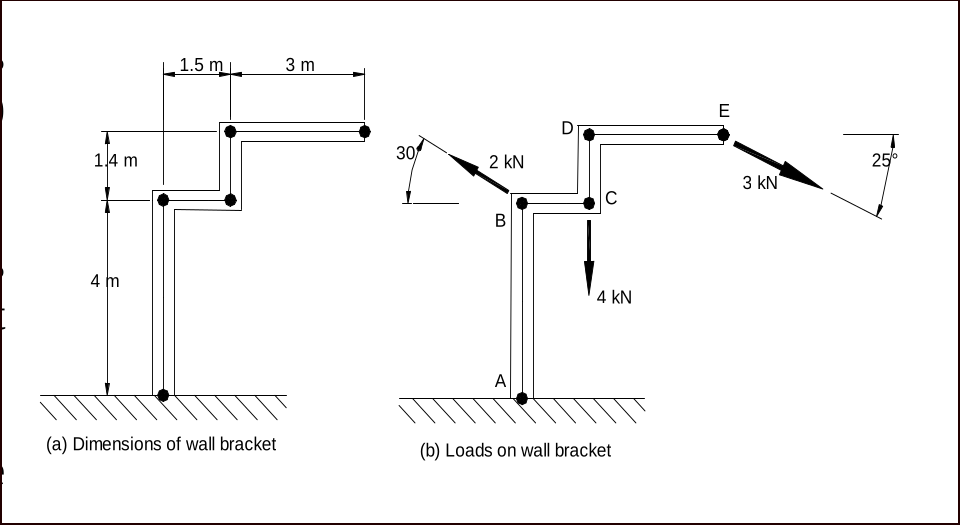
\includegraphics[scale=0.2]{topic-3}

Finding the moment around A
\begin{gather*}
    F_{2x} = 2\cos{30} \\ 
    F_{2y} = 2\sin{30} \\
    F_{4x} = 0 \\ 
    F_{4y} = -4 \\
    F_{3x} = 3\cos{25} \\
    F_{3y} = -3\sin{25} \\
    d_{2y} = 4m \\
    d_{2x} = 0m \\
    d_{4x} = 1.5m \\
    d_{4y} = 4m \\
    d_{3y} = 5.4m \\
    d_{3x} = 4.5m \\
    M_a = F_{2x} \cdot d_{2y} + F_{2y} \cdot d_{2x} + F_{4x} \cdot d_{4y} + F_{4y} \cdot d_{4x} + F_{3x} \cdot d_{3y} + F_{3y} \cdot d_{3x} \\
    M_a = F_{2x} \cdot d_{2y} + F_{4y} \cdot d_{4x} + F_{3x} \cdot d_{3y} + F_{3y} \cdot d_{3x} \\
    M_a = 2\cos{30} \cdot 4 + -4 \cdot 1.5 + 3\cos{25} \cdot 5.4 - 3\sin{25} \cdot 4.5 \\ 
    M_a = 19.46 \unit{kNm}
\end{gather*}
\subsection{Couples}
A couple is two forces that have equal magnitude but opposite direction, but that do not have the same line of action.
These forces sum to zero, but generate a moment. The value of a moment is simply the moments of the two forces subtracted from one another.
Or, alternatively, The magnitude of the two forces times by the distance between them. IMPORTANT NOTE: Couples have never been in a 121 exam before.

\end{document}
